\begin{algorithm}
\begin{algorithmic}[1]
    \State \textbf{Require:} \parbox[t]{\dimexpr\linewidth-\algorithmicindent}{perturbation function $q$\\ reconstruction function $r$ \strut}
    \State \textbf{Input:} \parbox[t]{\dimexpr\linewidth-\algorithmicindent}{Dataset $\D = \{(x_1, y_1)\ldots(x_n, y_n)\}$\\ number of augmented examples $m$ \strut}
    \Function{SSMBA}{$\D$, $m$}
    \State train a model $f$ on $\D$
    \For{$(x_i, y_i) \in \D$}
        \For{$j \in 1\ldots m$}
            \State sample perturbed $x_{ij}' \sim q(x'|x_i)$
            \State sample reconstructed $\hat{x}_{ij} \sim r(\hat{x}|x_{ij}')$ 
            \State generate $\hat{y}_{ij} \gets f(\hat{x}_{ij})$ or preserve \Statex[3] the original $y_i$
        \EndFor
    \EndFor
    \State let $\D^{aug} = \{(\hat{x}_{ij}, \hat{y}_{ij})\}_{i=1\ldots n,j=1\ldots m}$
    \State augment $ \D' \leftarrow \D \cup \D^{aug}$ 
    \State \Return $\D'$
    \EndFunction
\end{algorithmic}
\caption{SSMBA}
\label{alg:ssmba}
\end{algorithm}

\begin{figure}[t]
\centering
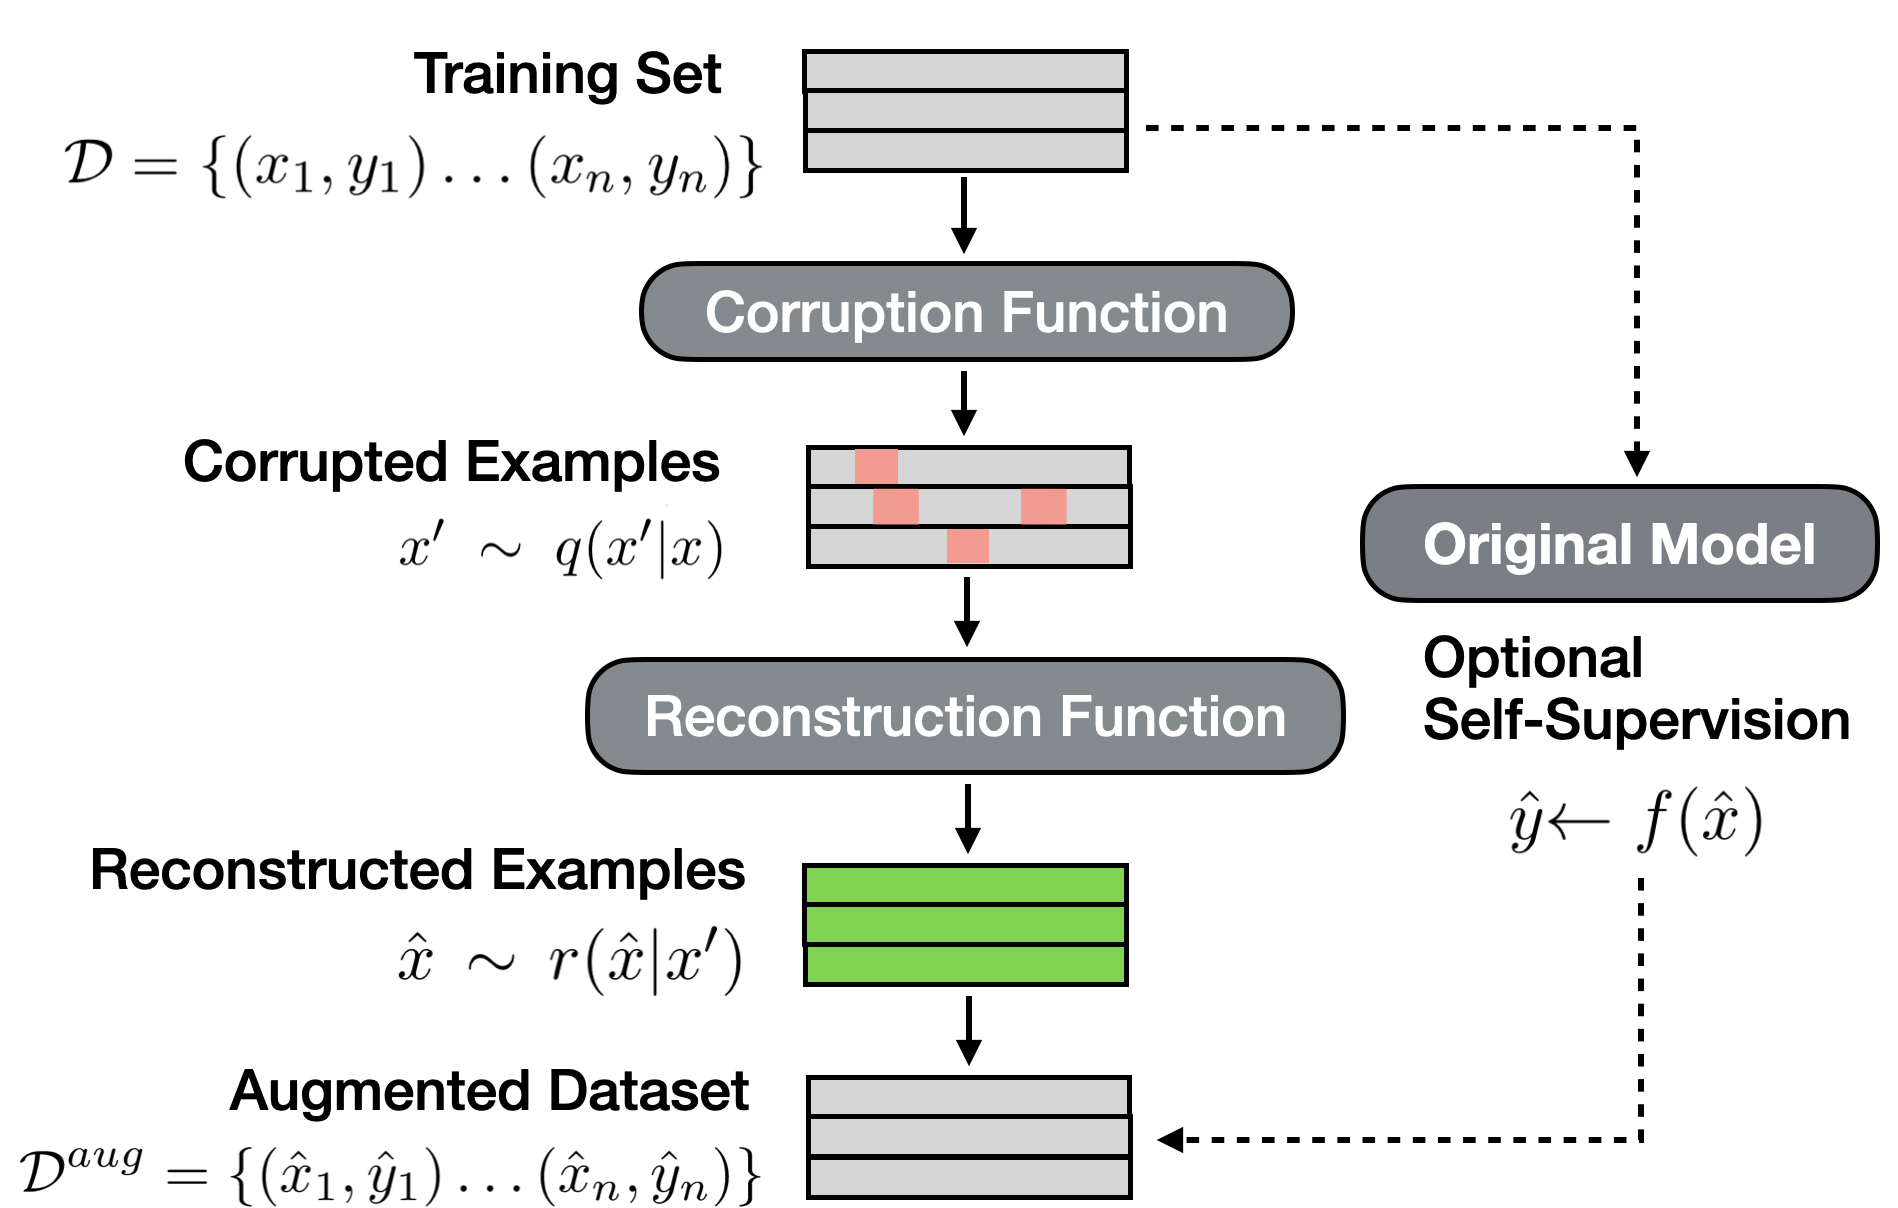
\includegraphics[scale=0.225]{img/ssmba_graph.png}
\caption{\ssmba\ generates synthetic examples by corrupting then reconstructing the original training inputs. 
To form the augmented dataset, corresponding outputs are preserved from the original data or generated from a supervised model $f$ trained on the original data.}
\label{fig:ssmba_graph}
\end{figure}

\noindent We now describe \textbf{S}elf-\textbf{S}upervised \textbf{M}anifold \textbf{B}ased Data \textbf{A}ugmentation. 
Let our original dataset $\D$ consist of pairs of input and output vectors $\D = \{(x_1, y_1)\ldots(x_n, y_n)\}$.
We assume the input points concentrate around an underlying lower dimensional data manifold $\M$.
Let $q$ be a corruption function from which we can draw a sample $x' \sim q(x'|x)$ such that $x'$ no longer lies on $\M$.
Let $r$ be a reconstruction function from which we can draw a sample $\hat{x} \sim r(\hat{x}|x')$ such that $\hat{x}$ lies on $\M$. 

To generate an augmented dataset, we take
each pair $(x_i, y_i)\in\D$ and sample a perturbed $x_i' \sim q(x'|x_i)$.
We then sample a reconstructed $\hat{x}_{ij} \sim r(\hat{x}|x_i')$.
A corresponding vector $\hat{y}_{ij}$ can be generated by preserving $y_i$, or, 
since examples in the manifold neighborhood may cross decision boundaries on more sensitive tasks, by using a teacher model trained on the original data.
This operation can be repeated to generate multiple augmented examples for each input example.
These new examples form a dataset that we can augment the original training set with. 
We can then train an augmented model on the new augmented dataset.

In this paper we investigate \ssmba's use on natural language tasks, using the MLM training corruption function as our corruption function $q$ and a pre-trained BERT model as our reconstruction model $r$.
Different from other data augmentation methods, %such as CBERT \citep{kobayashi-2018-contextual} and LAMBADA \citep{lambada}, 
\ssmba\ does not rely on task-specific knowledge, requires no dataset-specific fine-tuning, and is applicable to any supervised natural language task.
\ssmba\ requires only a pair of functions $q$ and $r$ used to generate data.

\comment{
\begin{figure*}[t!]
\centering
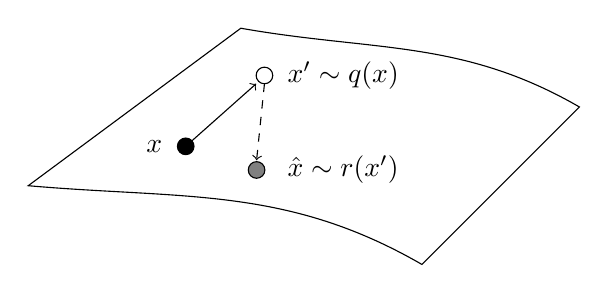
\begin{tikzpicture}

% we draw the surface
\draw (0,0) to[out=-5,in=150] (5,-1) -- (7,1) to[out=150,in=-10] (2.7,2.0) -- cycle;
\node at (6, 1) {$\M$};

% orginal point
\coordinate (x) at (2, 0.5);
\draw[fill] (x) circle (3pt);
\node at (1.6, 0.5) {$x$};

% perturbed point
\coordinate (qx) at (3, 1.4);
\draw (qx) circle (3pt);
\node at (4, 1.4) {$x' \sim q(x)$};

% reconstructed point
\coordinate(rqx) at (2.9, 0.2);
\draw[fill=gray] (rqx) circle (3pt);
\node at (4, 0.2) {$\hat{x} \sim r(x')$};

\draw [->] (x) -- ([xshift=-3pt,yshift=-3pt]qx);
\draw [dashed, ->] ([yshift=-3pt]qx) -- ([yshift=3.5pt]rqx);
\end{tikzpicture}
\caption{Noising and reconstruction process for a given point $x$ lying on a data manifold $\M$}
\end{figure*}
}